\documentclass[10pt]{article}
\usepackage{amsmath,amsfonts,times}
\usepackage{graphicx,color,tikz,pgfplots}
\usepackage[paperwidth=14cm,paperheight=5cm,lmargin=0in,rmargin=0in,tmargin=0.in,bmargin=0.in]{geometry}
\usepackage{bm}
\usetikzlibrary{arrows,shadings,shapes.arrows,decorations.pathreplacing,calc, positioning, shadows}
\usepgfplotslibrary{fillbetween}

\pgfplotsset{
  compat=newest
}

\newlength{\dx}
\setlength{\dx}{1cm}

\tikzset{
  node distance=1.0cm and 0.5cm,
  cell/.style={thick, draw=black},
  refined/.style={very thick, draw=black, solid, fill=blue, fill opacity=0.15},
  tree/.style={thick, draw=black},
  treenode/.style={draw=black, rounded corners=5pt,minimum width=8mm, minimum height=8mm, inner sep=1pt, fill=white, rectangle, very thick, drop shadow},
}

\begin{document}
\nopagecolor
\centering
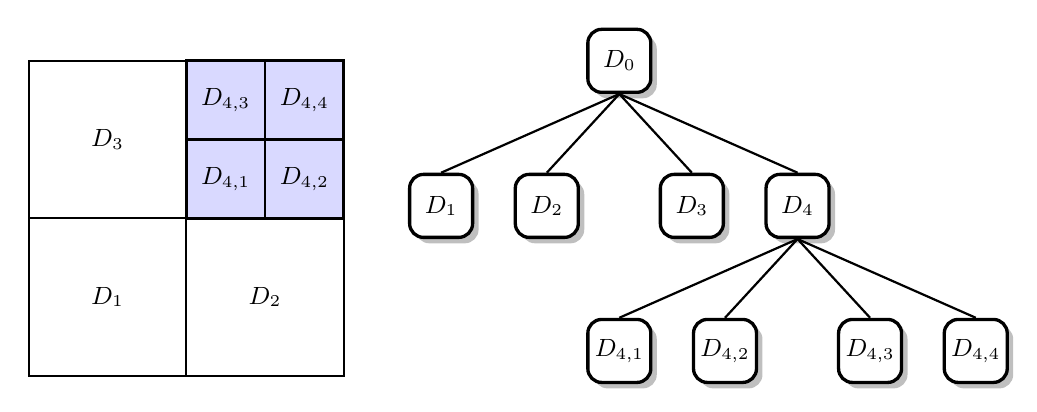
\begin{tikzpicture}[font=\small]

  % --- Spatial partitioning (a 2D quadtree, illustrating the same principle as a 3D octree) ---

  % Root cell, subdivided into 4 quadrants.
  \draw[cell] (0,0) rectangle (4\dx,4\dx);
  \draw[cell] (2\dx,0) -- (2\dx,4\dx);
  \draw[cell] (0,2\dx) -- (4\dx,2\dx);

  % Highlight the quadrant that is refined further.
  \draw[refined] (2\dx,2\dx) rectangle (4\dx,4\dx);

  % Second level of refinement inside that quadrant.
  \draw[cell] (3\dx,2\dx) -- (3\dx,4\dx);
  \draw[cell] (2\dx,3\dx) -- (4\dx,3\dx);

  \node at (1\dx,1\dx) {$D_1$};
  \node at (3\dx,1\dx) {$D_2$};
  \node at (1\dx,3\dx) {$D_3$};
  \node at (2.5\dx,2.5\dx) {\small $D_{4,1}$};
  \node at (3.5\dx,2.5\dx) {\small $D_{4,2}$};
  \node at (2.5\dx,3.5\dx) {\small $D_{4,3}$};
  \node at (3.5\dx,3.5\dx) {\small $D_{4,4}$};

  % --- Corresponding tree ---

  \node[treenode, alias=ROOT] at (7.5\dx, 4.0\dx) {$D_0$};
  \node[treenode, alias=C2, below left=of ROOT,anchor=north]  {$D_2$};
  \node[treenode, alias=C1, anchor=east, left=of C2.west]  {$D_1$};  
  \node[treenode, alias=C3, below right=of ROOT, anchor=north]  {$D_3$};
  \node[treenode, alias=C4, right=of C3.east,anchor=west]  {$D_4$};  

  \draw[tree] (ROOT.south) -- (C1.north);
  \draw[tree] (ROOT.south) -- (C2.north);
  \draw[tree] (ROOT.south) -- (C3.north);
  \draw[tree] (ROOT.south) -- (C4.north);


  \node[treenode, alias=G2, below left=of C4,anchor=north]{\small $D_{4,2}$};
  \node[treenode, alias=G1, left=of G2]{\small $D_{4,1}$};  
  \node[treenode, alias=G3, below right=of C4, anchor=north]{\small $D_{4,3}$};
  \node[treenode, alias=G4, right=of G3] {\small $D_{4,4}$};

  \draw[tree] (C4.south) -- (G1.north);
  \draw[tree] (C4.south) -- (G2.north);
  \draw[tree] (C4.south) -- (G3.north);
  \draw[tree] (C4.south) -- (G4.north);

\end{tikzpicture}

\end{document}
